\begin{apendicesenv}

\partapendices

  \chapter{Clusterização} \label{cap:clusterizacao}

A clusterização é denominada como técnica para organização ou agrupamento de uma coleção de padrões, ou elementos que sigam padrões, em \textit{clusters} baseada em similaridade.
Trata-se de uma técnica bastante utilizada em análise exploratórias, agrupamentos, tomada de decisão e implementações de \textit{machine learning}, como:
mineração de dados, recuperação de documentos, segmentação de imagens e padronização \cite{clustering_review}.

A aplicação da técnica pode ser resumida nos passos apresentados na Figura \ref{fig:tasks_clustering}.

\begin{figure}[h!]
\centering
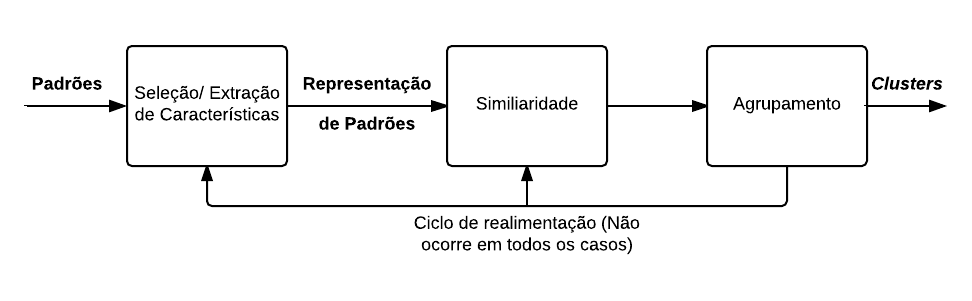
\includegraphics[scale=0.6]{figuras/tasks_clustering.png}
\caption{Passos para clusterização. Adaptado de \citeonline{clustering_review}}
\label{fig:tasks_clustering}
\end{figure}

A representação de padrões está relacionada ao número de classes, número de padrões disponíveis e o número, tipo e escala
das características disponíveis no algoritmo de clusterização. Algumas dessas informações podem não ser controladas pelos
profissionais \cite{clustering_review}.

A seleção de características é o processo de identificação do subconjunto das características mais eficaz para a clusterização, já a extração
de características é o uso de uma ou mais transformações das características de entrada para produzir novas características \cite{clustering_review}.

A similaridade, em geral, é medida por uma função de distância entre um par de padrões ou elementos. Essa função de distância pode variar
de acordo com o contexto da aplicação. E por fim, o agrupamento pode ser realizado com uso de vários algoritmos diferentes \cite{clustering_review}.

\section{Análise de \textit{clusters}}

\citeonline{tan2013data} definem a análise de \textit{clusters} como a ação que agrupa objetos de dados baseado apenas nas informações contidas
nos dados do próprio objeto que permitam descrever os objetos e suas relações. 

Classificação é o processo de encontrar um modelo que possa descrever e distinguir classes de dados \cite{han2011data}.

\citeonline{tan2013data}, \citeonline{han2011data} ressaltam a diferença entre classificação supervisionada e classificação não supervisionada.
Na classificação supervisionada os objetos de dados são analisados a partir de rótulos de classe predefinidos nos objetos, ou seja, 
com as classes de dados previamente definidas e conhecidas. \citeonline{han2011data} chamam este tipo de dado de "dado treinado"
(dados cujos rótulos são conhecidos), onde o modelo que o descreve é obtido a partir da análise dos rótulos.
Na classificação não supervisionada, os rótulos de classe são obtidos a partir da análise dos dados dos objetos, tão somente \cite{tan2013data}.

A clusterização geralmente se refere a este último tipo de classificação \cite{tan2013data}, onde os rótulos de classes dos objetos podem não existir ainda e 
o método empregado na clusterização pode gerar rótulos para um grupo de dados do conjunto \cite{han2011data}.

Os objetos são agrupados (ou "clusterizados") buscando maximizar a similaridade intraclasse e minimizar a similaridade interclasse.
Em outras palavras, o objetivo é formar \textit{clusters} cujos elementos tenham alta similaridade entre si em um mesmo \textit{cluster} 
e baixa similaridade a elementos de outros \textit{clusters} \cite{han2011data}. Por fim, um \textit{cluster} pode ser visto como uma
classe de objetos de onde se é possível derivar regras para o grupo \cite{han2011data}.

Apesar de parecer lógico e simples querer maximizar a similaridade intraclasse e minimizar a similaridade interclasse entre um conjunto de dados, 
\citeonline{tan2013data} exemplificam o quão difícil esta tarefa pode ser na Figura \ref{fig:clusters_difficulty}, onde temos um conjunto
de pontos (a) que pode ser agrupado de formas diferentes gerando quantidades diferentes de \textit{clusters} (b, c, d).

\begin{figure}[h!]
\centering
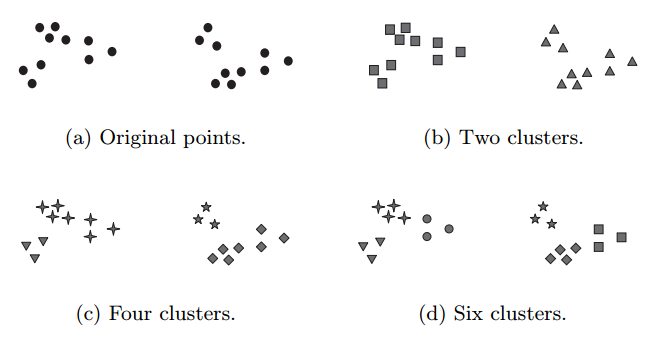
\includegraphics[scale=0.4]{figuras/clusters_difficulty.png}
\caption{Formas de se agrupar o mesmo conjunto de dados. Fonte: \cite{tan2013data}}
\label{fig:clusters_difficulty}
\end{figure}

 
\section{Tipos de clusterização}

\section{Algoritmos de clusterização}
  
% \chapter{Módulo matemático 0} \label{apd:kmeans}
% 
% Um módulo matemático implementado no ``Empurrando Juntos'' é baseado no algoritmo k-Means, apresentado no Capítulo \ref{cap:clusterizacao}. 
% 
% No ``Empurrando Juntos'' a entrada para os \textit{clusters} é a combinação entre participante,  
% comentário e o voto. Essa combinação gera uma entrada de N dimensões para N comentários.
% Frequentemente antes de medir a similaridade entre os objetos é necessário
% reduzir a dimensionalidade, isso acontece, pois para espaços de alta dimensão as distâncias euclidianas
% tendem a inflar. Reduzir a dimensionalidade pode aliviar esse problema e diminuir o tempo de cálculo.
% Um dos métodos mais utilizados para realizar essa redução é a Análise de 
% Componentes Principais (PCA, do inglês) \cite{han2011data, sklearn}.
% 
% \citeonline{mackiewicz1993principal} afirmam que a redução de dimensionalidade no PCA é
% obtida com a criação de uma nova combinação linear das variáveis que caracterizam os
% objetos estudados, satisfazendo condições matemáticas e estatísticas.
% \citeonline{shlens2014tutorial} afirma que o principal objetivo da técnica é identificar
% uma base para expressar um conjunto de dados que elimine os ruídos e revele 
% outros dados escondidos. 
% 
% \citeonline{han2011data} afirmam que o PCA 
% cria $k$ vetores ortogonais que possuem o mesmo significado que o conjunto
% de vetores inicial, porém trata-se de um conjunto menor. 
% 
% 
% A aplicação da técnica pode ser resumida nos seguintes passos listados abaixo.
% No final, os componentes principais restantes são uma boa aproximação dos 
% dados originais \cite{han2011data, mackiewicz1993principal, varella2008analise}: 
% 
% \begin{enumerate}
%  \item Criar uma matriz que represente os objetos estudados (n x p), onde as linhas representam cada objeto e as colunas representam as características;
%  \item Criar uma matriz de covariância (p x p) com os dados normalizados, caso as unidades sejam diferentes,
%   ara que eles estejam dentro da mesma variação;
%  \item Calcular os autovalores e autovetores da matriz de covariância, que 
%  são os componentes principais.
% \end{enumerate}
% 
% Além disso, foi aplicada uma técnica analítica para a definição do melhor valor para $k$, conhecida como Coeficiente de Silhueta \cite{sklearn}.
% 
% Essa técnica tem por objetivo combinar a avaliação de coesão e separação dos \textit{clusters} por meio do cálculo de um coeficiente (o de silhueta) que 
% varia de -1 a 1 e é dado pela fórmula \ref{eq:coeficiente} \cite{tan2013data}.
% 
% \begin{equation} \label{eq:coeficiente}
%   s_{i} = \frac{(b_{i} - a_{i})}{max(a_{i}, b_{i})} \mbox{, onde:}
% \end{equation}
% 
% {\addtolength{\leftskip}{8mm}
%     i é o objeto do \textit{cluster} que está sendo analisado
%     
%     $a_{i}$ é a média da distância entre o objeto e todos os objetos do seu \textit{cluster}
%     
%     $b_{i}$ é o valor mínimo da distância entre o objeto e os demais \textit{clusters}. 
%     
% 	  \footnotesize \indent \indent A distância entre o objeto e outro \textit{cluster} é média das distâncias entre o objeto \\ \indent \indent e todos os objetos do outro \textit{cluster}.
% }
% 
% Um coeficiente negativo representa que o elemento está no \textit{cluster} errado, pois isso significa que a distância entre o objeto e outro \textit{cluster} 
% é menor que a distância entre o objeto e os objetos de seu \textit{cluster}. O valor ``zero'' representa que o elemento está próximo da ``borda'' do \textit{cluster}, ou seja,
% a distância entre o objeto e outros \textit{clusters} e entre o objeto e os objetos de seu \textit{cluster} é a mesma. E por fim, quanto mais próximo do valor 1, melhor
% está a distribuição dos \textit{clusters}, pois significa que o valor de $a_i$ é menor que o valor de $b_i$.
% 
% Dessa forma, com a escolha de um intervalo de valores para $k$, como sugerido por \citeonline{han2011data} e \citeonline{sklearn}, é possível testar os valores 
% para o coeficiente de silhueta e escolher o melhor valor de $k$ dentro do intervalo. 
% 
% \begin{figure}[bt!]
% \centering
% 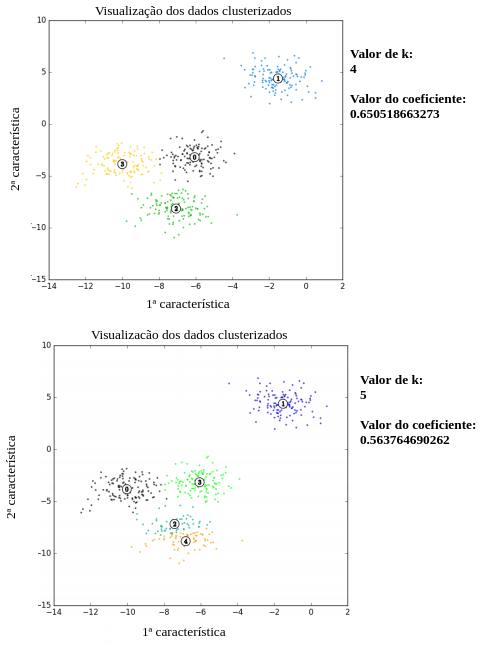
\includegraphics[scale=1]{figuras/exemplo_silhueta.png}
% \caption{Formação de \textit{clusters} utilizando K-means e seus coeficientes de silhueta. Adaptado de \citeonline{sklearn}}
% \label{fig:exemplo_silhueta}
% \end{figure}
% 
% \vfill
% \pagebreak
% Na Figura \ref{fig:exemplo_silhueta} é apresentado um exemplo visual de \textit{clusters} com diferentes valores
% de $k$ e seus coeficientes de silhueta.
% 
% Os métodos e técnicas apresentados fazem parte do algoritmo implementado no módulo de clusterização da plataforma 
% e possuem um objetivo específico. 
% 
% \begin{figure}[h!]
% \centering
% 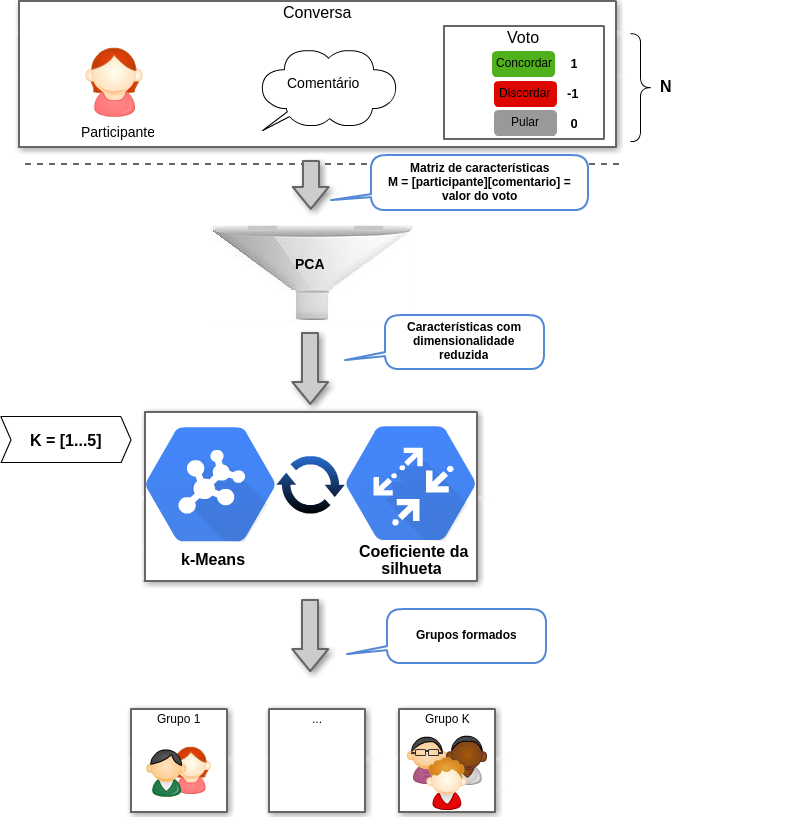
\includegraphics[scale=0.7]{figuras/resumo_clusterizao_ej.png}
% \caption{Fluxo de clusterização do ``Empurrando Juntos''}
% \label{fig:resumo_clusterizao_ej}
% \end{figure}
% 
% Quando o usuário cria uma conversa e outros participantes realizam comentários, para cada usuário é permitido realizar votos nesse comentários.
% Atualmente, a ideia é que o voto seja concordar, discordar ou pular. 
% 
% \vfill 
% \pagebreak
% A cada novo voto o fluxo apresentado na Figura \ref{fig:resumo_clusterizao_ej} é
% realizado. Para cada conversa, os N votos realizados nos N comentários são a entrada para o módulo de clusterização, 
% gerando uma entrada de dimensão N. A partir disso, é aplicada a técnica de PCA para que
% essa dimensionalidade seja reduzida. Com os dados em duas dimensões, é aplicada
% a técnica k-Means, para obtenção da disposição dos grupos de pessoas. O uso da técnica é
% feito em ciclos para a descoberta do melhor valor de $k$ por meio do cálculo do Coeficiente da silhueta.
% No final dos ciclos, a saída do fluxo são formados os grupos de pessoas com opiniões semelhantes.
% 
% O módulo de serviço, resultado deste trabalho, estabelece comunicação direta com este módulo de clusterização. 
% No módulo de serviço estão contidas todas as entidades que estabelecem os dados de entrada para a formação dos \textit{clusters}.

\end{apendicesenv}
